\section{Gaussian Process}
There are multiple ways of interpreting Gaussian Process models. In the following sections we want to highlight the function-space and weight-space interpretation which are both explained in more detail in \cite{GP_for_ML}. GPs can be applied both in regression and classification problems and stand out because of their inherent ability to associate an uncertainty measurement with every prediction.

\subsection{Function-Space Interpretation}
    In the function-space interpretation one can think of a GP as a distribution over functions, which is entirely defined by a mean function $m(x)$ and a covariance function $k(x,x')$. They are described by
        $$
        m(x) =\mathbb{E}[f(x)]
        $$
        $$
        k(x,x') = \mathbb{E}[(f(x)-m(x))(f(x')-m(x'))]
        $$
    and the GP is written as
        $$
        f({x}) \sim \mathcal{G} \mathcal{P}\left(m({x}), k\left({x}, {x}^{\prime}\right)\right).
        $$
    The prior and overall properties of this distribution depend on the covariance function. Examples of using different kernels as the covariance function and drawing function samples from the prior distribution can be seen in Figure~\ref{f:squared-exponential_prior} and Figure~\ref{f:ornstein_prior}.
    \begin{figure}[ht]
        \centering
        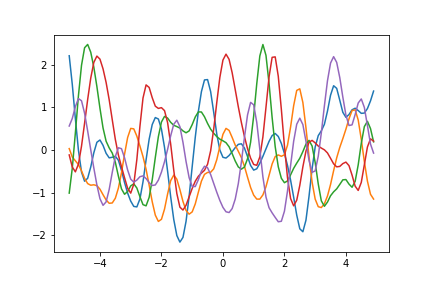
\includegraphics[width=.9\linewidth]{SoM_report_template/figures/prior.png}
        \caption[Prior with squared-exponential kernel]{\label{f:squared-exponential_prior}Function samples with squared-exponential kernel}
        \end{figure}
        \begin{figure}[ht]
        \centering
        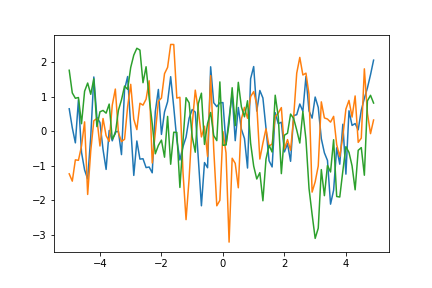
\includegraphics[width=.9\linewidth]{SoM_report_template/figures/priorornstein.png}
        \caption[Prior with Ornstein-Uhlenbeck kernel]{\label{f:ornstein_prior}Function samples with Ornstein-Uhlenbeck kernel}
    \end{figure}
    \newline
    The differences can obviously be large and the choice of $k(x,x')$ has to be made by assuming certain underlying properties of the system one would want to model. \newline
    
    To restrict the distribution over functions on functions that pass through known points the distribution can be conditioned on given data. This data consists of input values $X$ and function evaluations at these inputs $\mathbf f = f(X)$. One defines the data as $\mathcal{D}= \{\mathbf f,X\}$. This will allow drawing functions from the GP that comply with this data. An example can be seen in Figure~\ref{f:explfunction} where the known function evaluation are subject to some noise and $f(x)$ is unknown and to be found.
    \begin{figure}[ht]
        \centering
        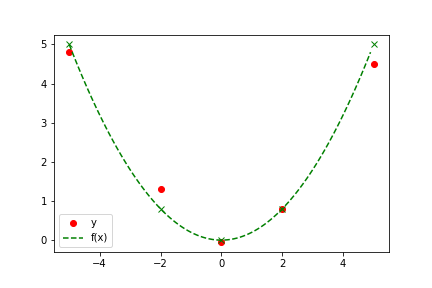
\includegraphics[width=.9\linewidth]{SoM_report_template/figures/function.png}
        \caption[Example function plot]{\label{f:explfunction}Noisy function evaluations $y$ of $f(x)=x^2$ in red.}
    \end{figure}
    To incorporate this knowledge we can write a joint Gaussian distribution between the given evaluations $\mathbb y$ and the unknown function values $\mathbb f_* := f(X_*)$. 
    \begin{equation} \begin{aligned}
    \label{eq:general_joint_gaussian}
        \footnotesize
        \setlength{\arraycolsep}{2.5pt}
        \medmuskip = 1mu % default: 4mu plus 2mu minus 4mu
        \scriptstyle
            \left[\begin{array}{c}
            \mathbf{y} \\
            \mathbf{f}_{*}
            \end{array}\right] \sim \mathcal{N}\left(\mathbf{0},\left[\begin{array}{cc}
            K(X, X)+\sigma_{n}^{2} I & K\left(X, X_{*}\right) \\
            K\left(X_{*}, X\right) & K\left(X_{*}, X_{*}\right)
            \end{array}\right]\right) \end{aligned}
    \end{equation}
    Here we inherently assume that function evaluations at \textit{close} $x$-values should result in \textit{close} function values $f(x)$. The distance is described by the covariance function $k(x,x')$ that describes how \textit{close} some points are. The term $+\sigma_{n}^{2}$ in (\ref{eq:general_joint_gaussian}) results in a covariance larger than zero for all the given function values, which implies that a certain noise is assumed in the data. This means we assume a relation $y = f(x) +\epsilon$ where $\epsilon$ is sampled from some probability density function (pdf). Setting $\sigma$ to zero will result in function samples that perfectly pass through the given data. By using the rules for finding the conditional distribution of a multivariate Gaussian one can find the mean $\mu (x)$ and variance $\Sigma(x)$ of that conditional at $x_*$ to be
    \begin{equation}
        \label{eq:GPmean}
        \mu(x_*) := 
        \mathbb{E}_{f_*}\left[\mathbf{f}_{*}|D\right] = 
        k_*^T[K+\sigma ^{2} I]^{-1} \mathbf{y}
    \end{equation}
    \begin{equation}
        \label{eq:GPvariance}
        \Sigma(x_*):=
        \mathbb{V}_{f_*}\left[\mathbf{f}_{*}|D\right] =
        k\left(x_{*}, x_{*}\right)-k_*^T\left(K+\sigma ^{2} I\right)^{-1} k_*
    \end{equation}
    where $k_* = k(x_*,X)^T$ and $K = k(X,X)$ for notational simplicity. Plotting the resultant mean and variance for the example in Figure~\ref{f:explfunction} with different kernel functions can be seen in Figure~\ref{f:interfunction}.
    \begin{figure}[ht]
        \centering
        \subfigure[Squared-exponential kernel]{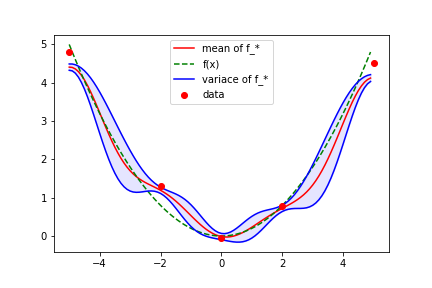
\includegraphics[width=0.9\linewidth]{SoM_report_template/figures/posterior.png}}\quad
        \subfigure[Ornstein-Uhlenbeck kernel]{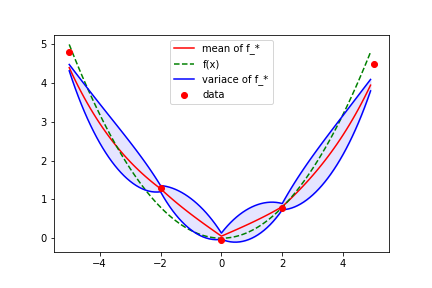
\includegraphics[width=0.9\linewidth]{SoM_report_template/figures/posteriororn.png}}
        \caption[Posterior distribution examples]{\label{f:interfunction}Posterior function distributions for different kernel functions}
    \end{figure}
    \newline
    To quantify how good the fit actually is the \textit{marginal likelihood} $p(\mathbb y|X)$ can be used. It can be computed with the integral
    $$
    p(\mathbf{y} \mid X)=\int p(\mathbf{y} \mid \mathbf{f}, X) p(\mathbf{f} \mid X) d \mathbf{f}
    $$
    that quantifies how likely the noisy measurements $y$ are as function evaluations at $X$ with the current model. Taking the logarithm allows for easier optimization and results in 
    \begin{align*}
        \log p(\mathbf{y} \mid X)=-\frac{1}{2} \mathbf{y}^{\top}\left(K+\sigma_{n}^{2} I\right)^{-1} \\ \mathbf{y}-\frac{1}{2} \log \left|K+\sigma_{n}^{2} I\right|-\frac{n}{2} \log 2 \pi
    \end{align*}
    for the GP formulation.
    \newpage
\subsection{Weight-Space Interpretation}
    As the GP describes a distribution of functions one can write it as a possibly infinite linear combination of functions. This can be written as
    \begin{equation}
        \label{eq:weight-spacef}
        f(x) = \phi(x)^T \mathbb \theta
    \end{equation}
    Sampling from the prior is easy here. It just requires sampling the required weights $\theta \sim \mathcal N (0,\Sigma_p)$. This is a property that will later in this report be of great use. The posterior can be drawn from the distribution
    \begin{equation}
        \begin{split}
        f_{*} \mid {x}_{*}, X, {y} \sim  \mathcal{N}\left(\frac{1}{\sigma_{n}^{2}} \phi\left({x}_{*}\right)^{\top} A^{-1} \Phi {y},\\ \phi\left({x}_{*}\right)^{\top} A^{-1} \phi\left({x}_{*}\right)\right).
        \end{split}
    \end{equation}
    where $\Phi = \phi(X)$ and $A = \sigma_{n}^{-2} \Phi \Phi^{\top}+\Sigma_{p}^{-1}$
